\documentclass[11pt]{article}
\usepackage[UTF8]{ctex}
\usepackage[a4paper,left=25mm,right=25mm,top=25mm]{geometry}
\usepackage{xeCJKfntef}
\usepackage{amsmath,amsfonts,amssymb}
\usepackage{tikz}
\usepackage{pifont}
\usepackage{subfigure}
\usepackage{caption}
\usetikzlibrary{arrows.meta}
\renewcommand{\figurename}{}
\renewcommand{\thesubfigure}{(\arabic{subfigure})}
\makeatletter \renewcommand{\@thesubfigure}{\thesubfigure \space}
\renewcommand{\p@subfigure}{} \makeatother
\begin{document}
\begin{figure}[h]
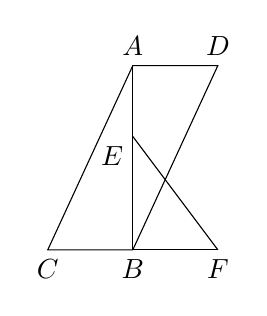
\begin{tikzpicture}[scale=0.18]
    \node[above] at (0,13) {$A$};
    \node[below] at (0,0) {$B$};
    \node[below] at (-6,0) {$C$};
    \node[below] at (6,0) {$F$};
    \node[above] at (6,13) {$D$};
    \node[below left] at (0,8) {$E$};
    \draw (-6,0)--(0,13)--(6,13)--(0,0)--cycle;
    \draw (0,13)--(0,0);
    \draw (0,0)--(6,0);
    \draw (0,8)--(6,0);
\end{tikzpicture}
\end{figure}
\end{document}